% Options for packages loaded elsewhere
\PassOptionsToPackage{unicode}{hyperref}
\PassOptionsToPackage{hyphens}{url}
%
\documentclass[
]{article}
\usepackage{amsmath,amssymb}
\usepackage{iftex}
\ifPDFTeX
  \usepackage[T1]{fontenc}
  \usepackage[utf8]{inputenc}
  \usepackage{textcomp} % provide euro and other symbols
\else % if luatex or xetex
  \usepackage{unicode-math} % this also loads fontspec
  \defaultfontfeatures{Scale=MatchLowercase}
  \defaultfontfeatures[\rmfamily]{Ligatures=TeX,Scale=1}
\fi
\usepackage{lmodern}
\ifPDFTeX\else
  % xetex/luatex font selection
\fi
% Use upquote if available, for straight quotes in verbatim environments
\IfFileExists{upquote.sty}{\usepackage{upquote}}{}
\IfFileExists{microtype.sty}{% use microtype if available
  \usepackage[]{microtype}
  \UseMicrotypeSet[protrusion]{basicmath} % disable protrusion for tt fonts
}{}
\makeatletter
\@ifundefined{KOMAClassName}{% if non-KOMA class
  \IfFileExists{parskip.sty}{%
    \usepackage{parskip}
  }{% else
    \setlength{\parindent}{0pt}
    \setlength{\parskip}{6pt plus 2pt minus 1pt}}
}{% if KOMA class
  \KOMAoptions{parskip=half}}
\makeatother
\usepackage{xcolor}
\usepackage[margin=1in]{geometry}
\usepackage{color}
\usepackage{fancyvrb}
\newcommand{\VerbBar}{|}
\newcommand{\VERB}{\Verb[commandchars=\\\{\}]}
\DefineVerbatimEnvironment{Highlighting}{Verbatim}{commandchars=\\\{\}}
% Add ',fontsize=\small' for more characters per line
\usepackage{framed}
\definecolor{shadecolor}{RGB}{248,248,248}
\newenvironment{Shaded}{\begin{snugshade}}{\end{snugshade}}
\newcommand{\AlertTok}[1]{\textcolor[rgb]{0.94,0.16,0.16}{#1}}
\newcommand{\AnnotationTok}[1]{\textcolor[rgb]{0.56,0.35,0.01}{\textbf{\textit{#1}}}}
\newcommand{\AttributeTok}[1]{\textcolor[rgb]{0.13,0.29,0.53}{#1}}
\newcommand{\BaseNTok}[1]{\textcolor[rgb]{0.00,0.00,0.81}{#1}}
\newcommand{\BuiltInTok}[1]{#1}
\newcommand{\CharTok}[1]{\textcolor[rgb]{0.31,0.60,0.02}{#1}}
\newcommand{\CommentTok}[1]{\textcolor[rgb]{0.56,0.35,0.01}{\textit{#1}}}
\newcommand{\CommentVarTok}[1]{\textcolor[rgb]{0.56,0.35,0.01}{\textbf{\textit{#1}}}}
\newcommand{\ConstantTok}[1]{\textcolor[rgb]{0.56,0.35,0.01}{#1}}
\newcommand{\ControlFlowTok}[1]{\textcolor[rgb]{0.13,0.29,0.53}{\textbf{#1}}}
\newcommand{\DataTypeTok}[1]{\textcolor[rgb]{0.13,0.29,0.53}{#1}}
\newcommand{\DecValTok}[1]{\textcolor[rgb]{0.00,0.00,0.81}{#1}}
\newcommand{\DocumentationTok}[1]{\textcolor[rgb]{0.56,0.35,0.01}{\textbf{\textit{#1}}}}
\newcommand{\ErrorTok}[1]{\textcolor[rgb]{0.64,0.00,0.00}{\textbf{#1}}}
\newcommand{\ExtensionTok}[1]{#1}
\newcommand{\FloatTok}[1]{\textcolor[rgb]{0.00,0.00,0.81}{#1}}
\newcommand{\FunctionTok}[1]{\textcolor[rgb]{0.13,0.29,0.53}{\textbf{#1}}}
\newcommand{\ImportTok}[1]{#1}
\newcommand{\InformationTok}[1]{\textcolor[rgb]{0.56,0.35,0.01}{\textbf{\textit{#1}}}}
\newcommand{\KeywordTok}[1]{\textcolor[rgb]{0.13,0.29,0.53}{\textbf{#1}}}
\newcommand{\NormalTok}[1]{#1}
\newcommand{\OperatorTok}[1]{\textcolor[rgb]{0.81,0.36,0.00}{\textbf{#1}}}
\newcommand{\OtherTok}[1]{\textcolor[rgb]{0.56,0.35,0.01}{#1}}
\newcommand{\PreprocessorTok}[1]{\textcolor[rgb]{0.56,0.35,0.01}{\textit{#1}}}
\newcommand{\RegionMarkerTok}[1]{#1}
\newcommand{\SpecialCharTok}[1]{\textcolor[rgb]{0.81,0.36,0.00}{\textbf{#1}}}
\newcommand{\SpecialStringTok}[1]{\textcolor[rgb]{0.31,0.60,0.02}{#1}}
\newcommand{\StringTok}[1]{\textcolor[rgb]{0.31,0.60,0.02}{#1}}
\newcommand{\VariableTok}[1]{\textcolor[rgb]{0.00,0.00,0.00}{#1}}
\newcommand{\VerbatimStringTok}[1]{\textcolor[rgb]{0.31,0.60,0.02}{#1}}
\newcommand{\WarningTok}[1]{\textcolor[rgb]{0.56,0.35,0.01}{\textbf{\textit{#1}}}}
\usepackage{graphicx}
\makeatletter
\def\maxwidth{\ifdim\Gin@nat@width>\linewidth\linewidth\else\Gin@nat@width\fi}
\def\maxheight{\ifdim\Gin@nat@height>\textheight\textheight\else\Gin@nat@height\fi}
\makeatother
% Scale images if necessary, so that they will not overflow the page
% margins by default, and it is still possible to overwrite the defaults
% using explicit options in \includegraphics[width, height, ...]{}
\setkeys{Gin}{width=\maxwidth,height=\maxheight,keepaspectratio}
% Set default figure placement to htbp
\makeatletter
\def\fps@figure{htbp}
\makeatother
\setlength{\emergencystretch}{3em} % prevent overfull lines
\providecommand{\tightlist}{%
  \setlength{\itemsep}{0pt}\setlength{\parskip}{0pt}}
\setcounter{secnumdepth}{-\maxdimen} % remove section numbering
\usepackage{booktabs}
\usepackage{longtable}
\usepackage{array}
\usepackage{multirow}
\usepackage{wrapfig}
\usepackage{float}
\usepackage{colortbl}
\usepackage{pdflscape}
\usepackage{tabu}
\usepackage{threeparttable}
\usepackage{threeparttablex}
\usepackage[normalem]{ulem}
\usepackage{makecell}
\usepackage{xcolor}
\ifLuaTeX
  \usepackage{selnolig}  % disable illegal ligatures
\fi
\usepackage{bookmark}
\IfFileExists{xurl.sty}{\usepackage{xurl}}{} % add URL line breaks if available
\urlstyle{same}
\hypersetup{
  pdftitle={Data exploration of the immune response of wild mice against parasite infections},
  pdfauthor={Fay},
  hidelinks,
  pdfcreator={LaTeX via pandoc}}

\title{Data exploration of the immune response of wild mice against
parasite infections}
\author{Fay}
\date{2024-02-01}

\begin{document}
\maketitle

\section{Data structure of field and laboratory data
sets}\label{data-structure-of-field-and-laboratory-data-sets}

\subsection{Data originating from yearly field excursions in the House
Mouse Hybrid
Zone}\label{data-originating-from-yearly-field-excursions-in-the-house-mouse-hybrid-zone}

GitHub repository:
\url{https://github.com/derele/Mouse_Eimeria_Field/tree/master}

\subsubsection{Infection intensity data}\label{infection-intensity-data}

\emph{Eimeria spp.} oocysts counting:

counter: character, Person who counted Feces\_g: numeric, amount of
feces used in flotation Date\_count: date counted N\_oocysts\_sq1
\ldots{} sq8: numeric, individual count for each single square on the
neubaure chamber (up to 8) mean\_neubauer: numeric, mean of the 8
squares PBS\_dil\_in\_mL: numeric, in which volume of PBS whas Ncells:
number of neubauer ``cells'' (squares) counted OPG: oocysts per gram
feces (calculated from the above) In some cases only OPG data might be
available or rather data would need to be re-formatted to access all the
raw values.

\emph{Eimeria spp.} detection qPCR We perform relative qPCR for
detection and quantification of Eimeria DNA in intestinal tissue. We
amplify a locus in the nuclear genome of the house mouse and a locus in
the mitochondrial genome (COI) of Eimeria. We then calculate a ``delta''
between the two ct values.

delta\_ct\_ilwe\_MminusE: threshold cycle for mouse minus Eimeria in
Ileum tissue. Only E. vermiformis is (at low pervalence in Ileum tissue)
and we therefore don't obtain this data-type for all years.

delta\_ct\_cewe\_MminusE: threshold cycle for mouse minus Eimeria in
Caecume tissue. E. ferrisi and E. falcifromis are detected here. We
should have this (as coprehensively as possible) for every year!

MC.Eimeria: TRUE/FALSE. This was established in 2018 as an improvement
over the `\textgreater{} -5 delta ct rule' for identification of Eimeria
-positive qPCRs. Melting curves have to show a drastic drop at XX°C to
indicate melting of a proper Eimeria COI amplification product. It might
be added where possible for per 2018 data post-hoc (if melting curves
exist for a review of raw data).

\subsection{\texorpdfstring{Data structure - laboratory challenge
infections with \emph{Eimeria
spp.}}{Data structure - laboratory challenge infections with Eimeria spp.}}\label{data-structure---laboratory-challenge-infections-with-eimeria-spp.}

Contains data for challenge (repeated) infections performed between 2017
and 2019. The data product is structure in the following columns:

Mouse\_ID: the unique identifier of the mouse experiment: the experiment
as numbered in the overview table mouse\_strain: the strain (inbred or
outbred) of the mouse primary\_infection: The Eimeria strain used for
the primary infection challenge\_infection: The Eimeria strain used for
the challenge infection infection\_history: The resulting infection
history labels: the unique label of the fecal sample at a particular dpi
weight: the weight of the mouse at this dpi weight\_dpi0: the weight at
the day of infection relative\_weight: the weight of the mouse at this
dpi relative to the weight at dpi0 feces\_weight: the weight of the
feces collected at this dpi dpi: days post infection at which samples
and data in this row were taken infection: the infection (primary or
challenge) this row/dpi corresponds to oocyst\_sq1, oocyst\_sq2,
oocyst\_sq3, oocyst\_sq4: the raw values for squared during oocyst
counting dilution: the amount of PBS the feces (with it's relative
weight) was dissolved in OO4sq: the sum of oocysts in the four counting
squares OOC: the overall number of oocysts in in the feces (of a
particular weight) at this dpi OPG\_O: Old way of counting opg (Emanuel
ask me) infection\_type: what kind of infection are we looking at
(challenge or primary, homologous or heterologous immunization). This is
differently coded to infection, as here UNI:E88 (first uninfected, then
infected with E88) would count as a ``primaryE88'' infection The next
values max\_dpi until maximum\_weight are calculated for the infection
type in which the mice died

max\_dpi = maximum dpi that the mouse that the mouse reached for each
infection challenge or primary (group\_by EH\_ID and infection
(primary/challenge) to get the value

maximum oocysts for each infection type (group\_by EH\_ID and infection
(primary/challenge) to get the value)

maximum weight loss for each infection type (group\_by EH\_ID and
infection (primary/challenge) to get the value)

death = challenge/primary (in which infection did the mouse die

Eim\_MC = Melting curve for eimeria

delta = delta ct value

\section{Experimental planning - Laboratory
infections}\label{experimental-planning---laboratory-infections}

\subsection{Selected mouse strains}\label{selected-mouse-strains}

\begin{itemize}
\tightlist
\item
  four wild-derived inbred mouse strains along with their respective F1
  hybrids.
\item
  Two of these strains, SCHUNT and STRA, represent M. m. domesticus.
\item
  The strains BUSNA and PWD were derived from M. m. musculus
\item
  Two intersubspecific hybrids (STRAxBUSNA and SCHUNTxPWD) and
\item
  Two intrasubspecific hybrids (SCHUNTxSTRA and PWDxBUSNA).
\end{itemize}

\begin{tabular}{l|l}
\hline
  & hybrid\_status\\
\hline
SCHUNT & M. m. domesticus\\
\hline
STRA & M. m. domesticus\\
\hline
BUSNA & M. m. musculus\\
\hline
PWD & M. m. musculus\\
\hline
STRA BUSNA & intersubspecific hybrids\\
\hline
SCHUNT PWD & intersubspecific hybrids\\
\hline
SCHUNT STRA & intrasubspecific hybrids\\
\hline
PWD BUSNA & intrasubspecific hybrids\\
\hline
\end{tabular}

Numbers of each mouse strain

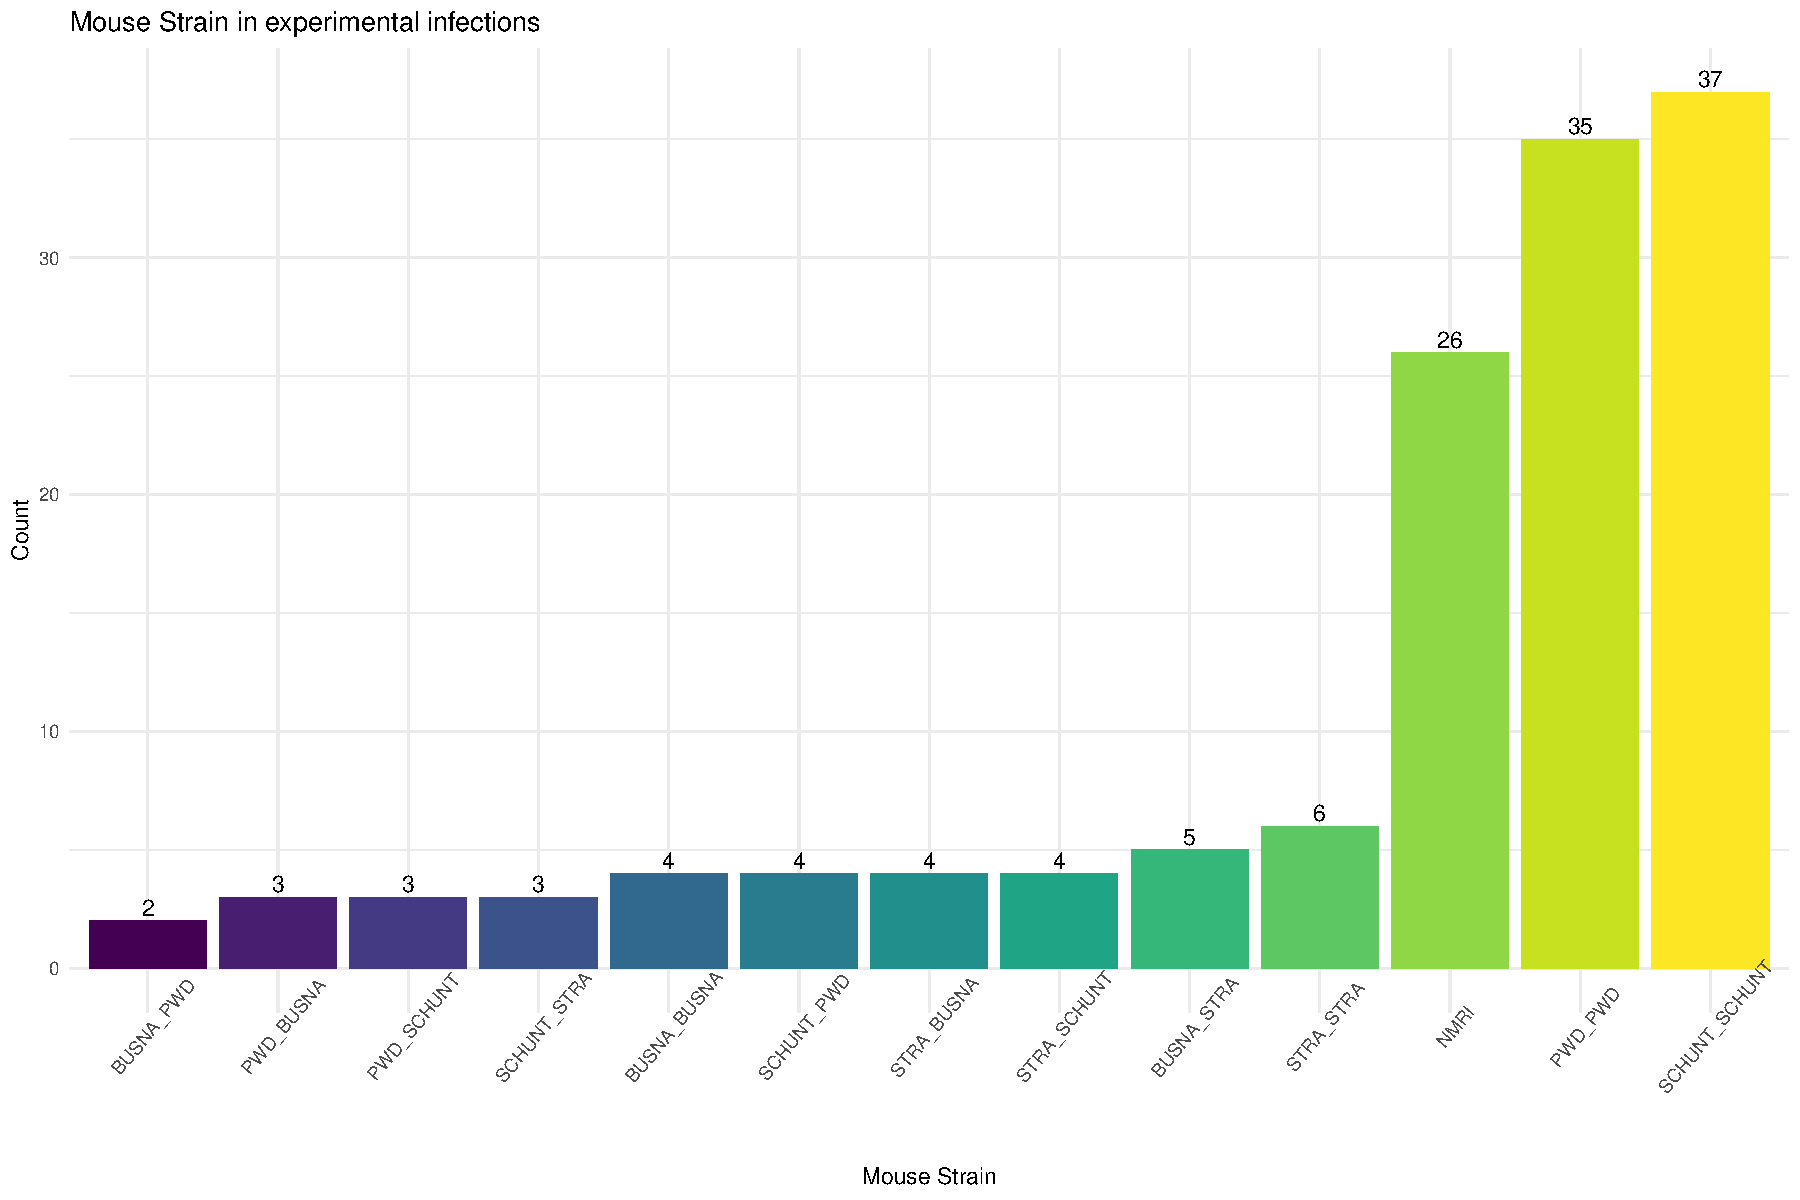
\includegraphics{Explorative_Stats_experimental_planning_files/figure-latex/strains-1.pdf}

\subsection{Selected parasite strains}\label{selected-parasite-strains}

Infections were initiated by oral administration of 150 sporulated
Eimeria oocysts * Up to 16 species of Eimeria have been described from
house mice * Overall prevalence in the wild 25.9\% * Prevalence of
\emph{E. ferrisi} 14 \% * Prevalence of \emph{E. falciformis} 4\%

As a proxy for health we use the maximum relative weight lost during
infection

Maximum weight loss = highest relative weight on any day of the
experiment / starting weight

\subsection{Maximum relative weight loss in each infection group, in
challenge and primary infections
combined.}\label{maximum-relative-weight-loss-in-each-infection-group-in-challenge-and-primary-infections-combined.}

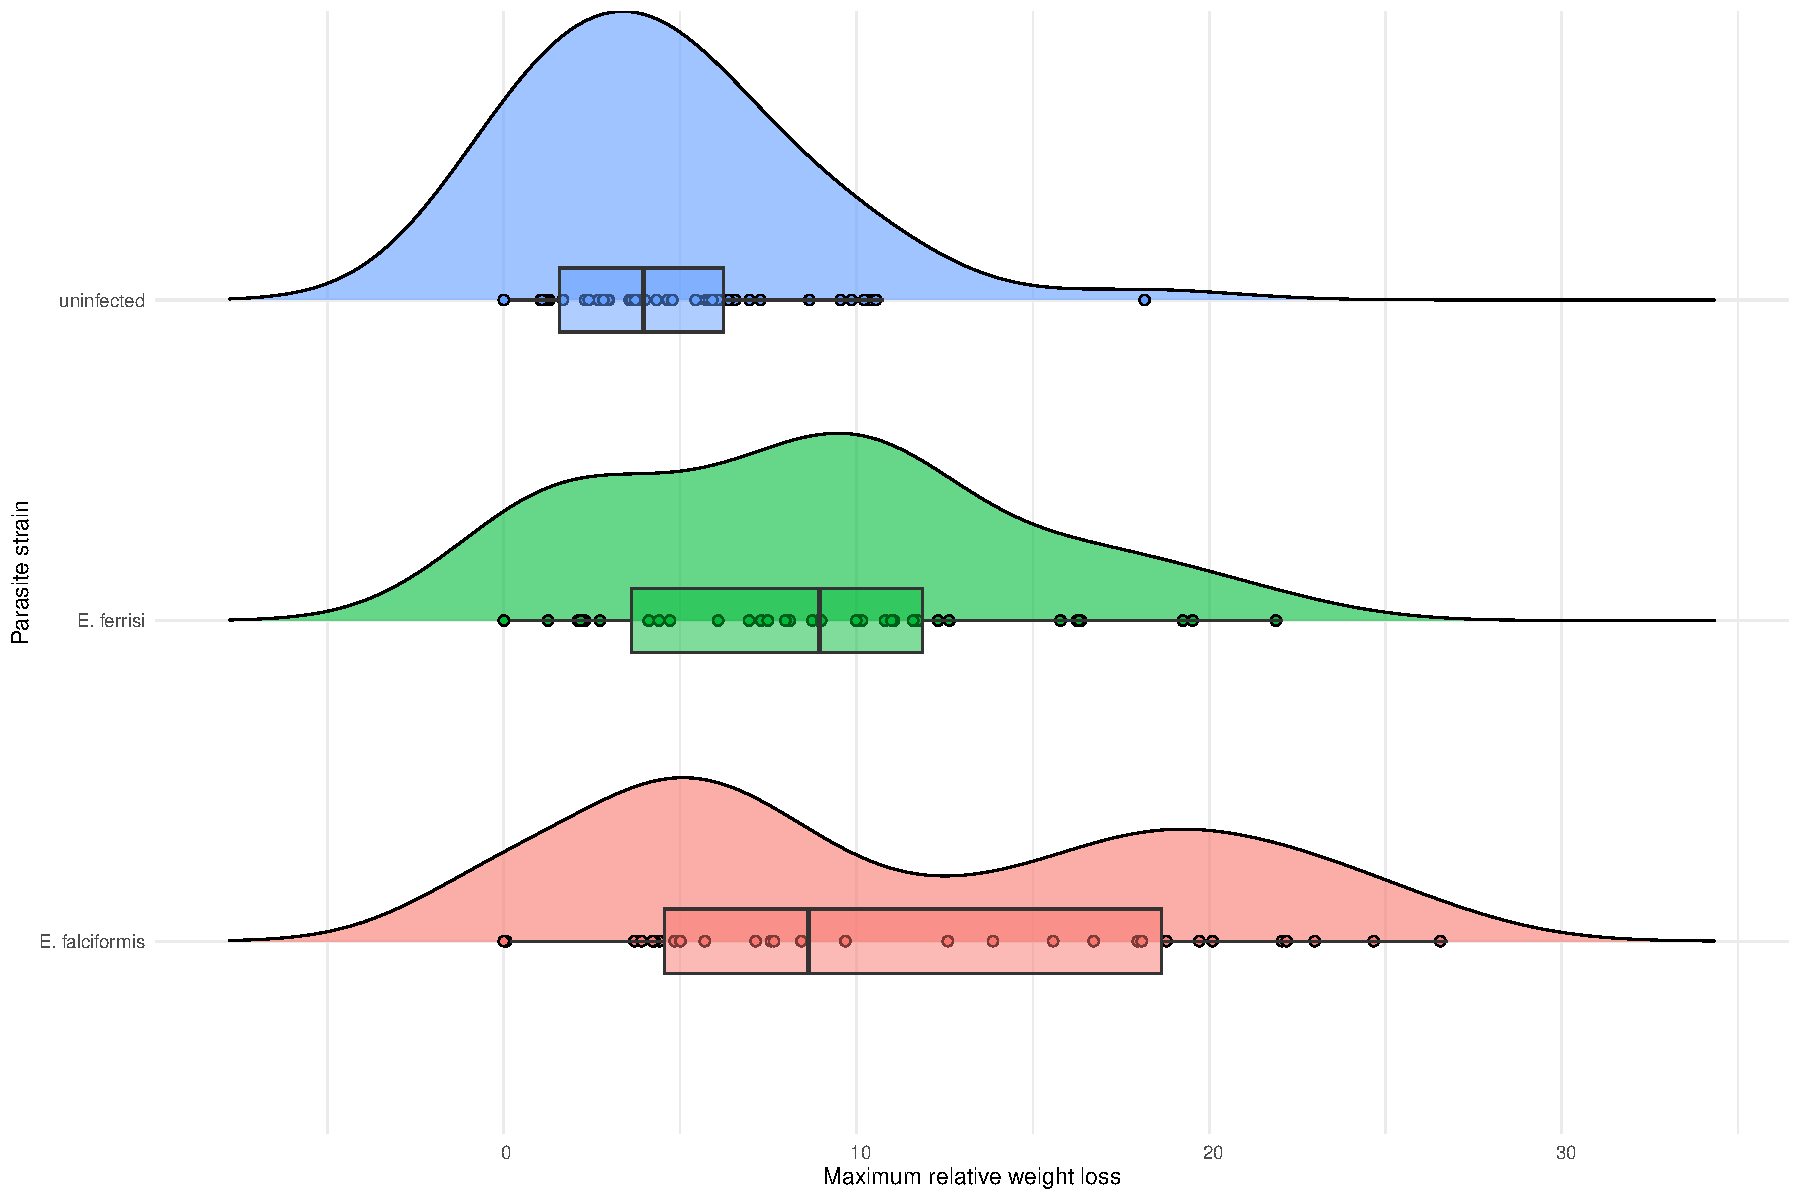
\includegraphics{Explorative_Stats_experimental_planning_files/figure-latex/general_WL_parasite-1.pdf}

Most of the mice in this experiment, are mice that have been challenged
(infected for a second time). This replicates more accurately what
happens in the wild. A much higher weight loss is expected in the
primary infections.

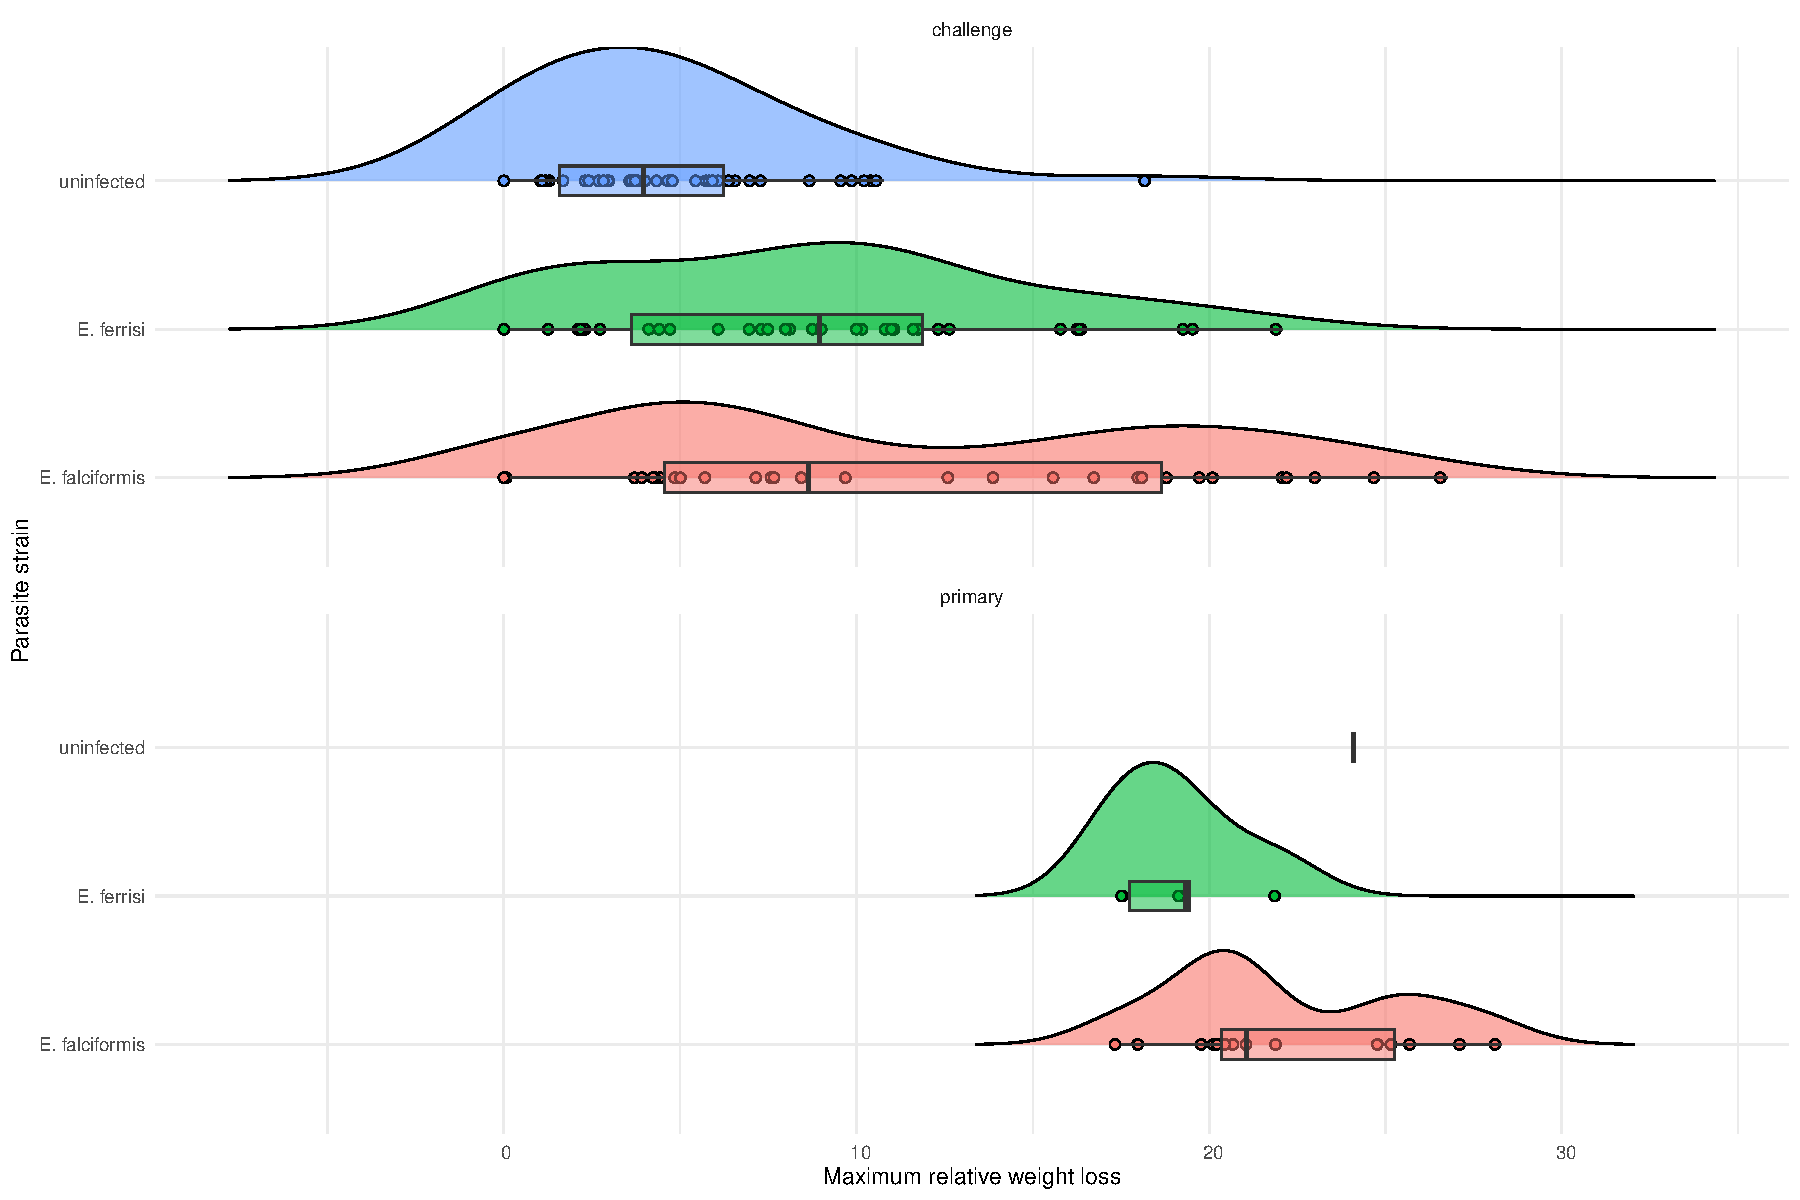
\includegraphics{Explorative_Stats_experimental_planning_files/figure-latex/general_WL_parasite_infection-1.pdf}

\subsection{Weight loss per mouse
strain}\label{weight-loss-per-mouse-strain}

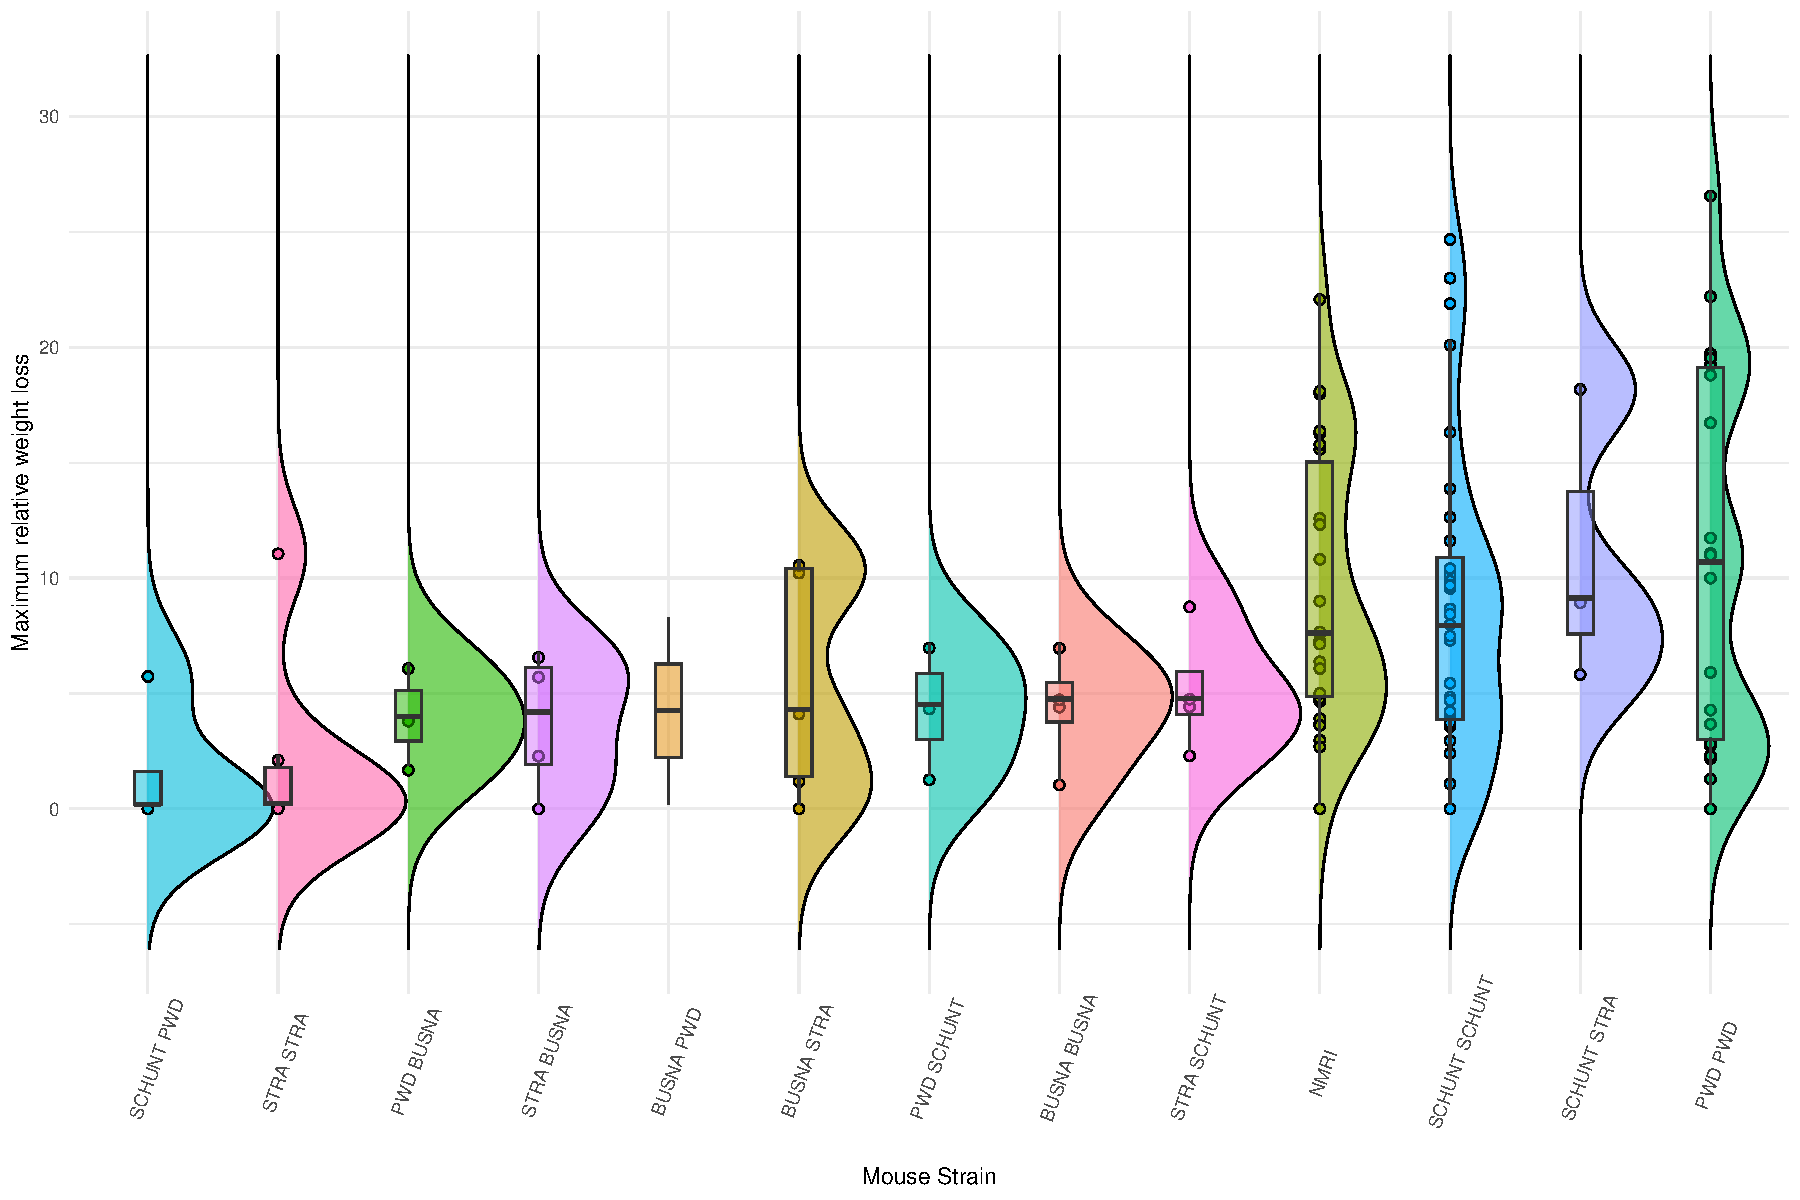
\includegraphics{Explorative_Stats_experimental_planning_files/figure-latex/mouse_strain_WL-1.pdf}

\subsubsection{Weight loss per mouse strain, challenge infections vs
primary
infections}\label{weight-loss-per-mouse-strain-challenge-infections-vs-primary-infections}

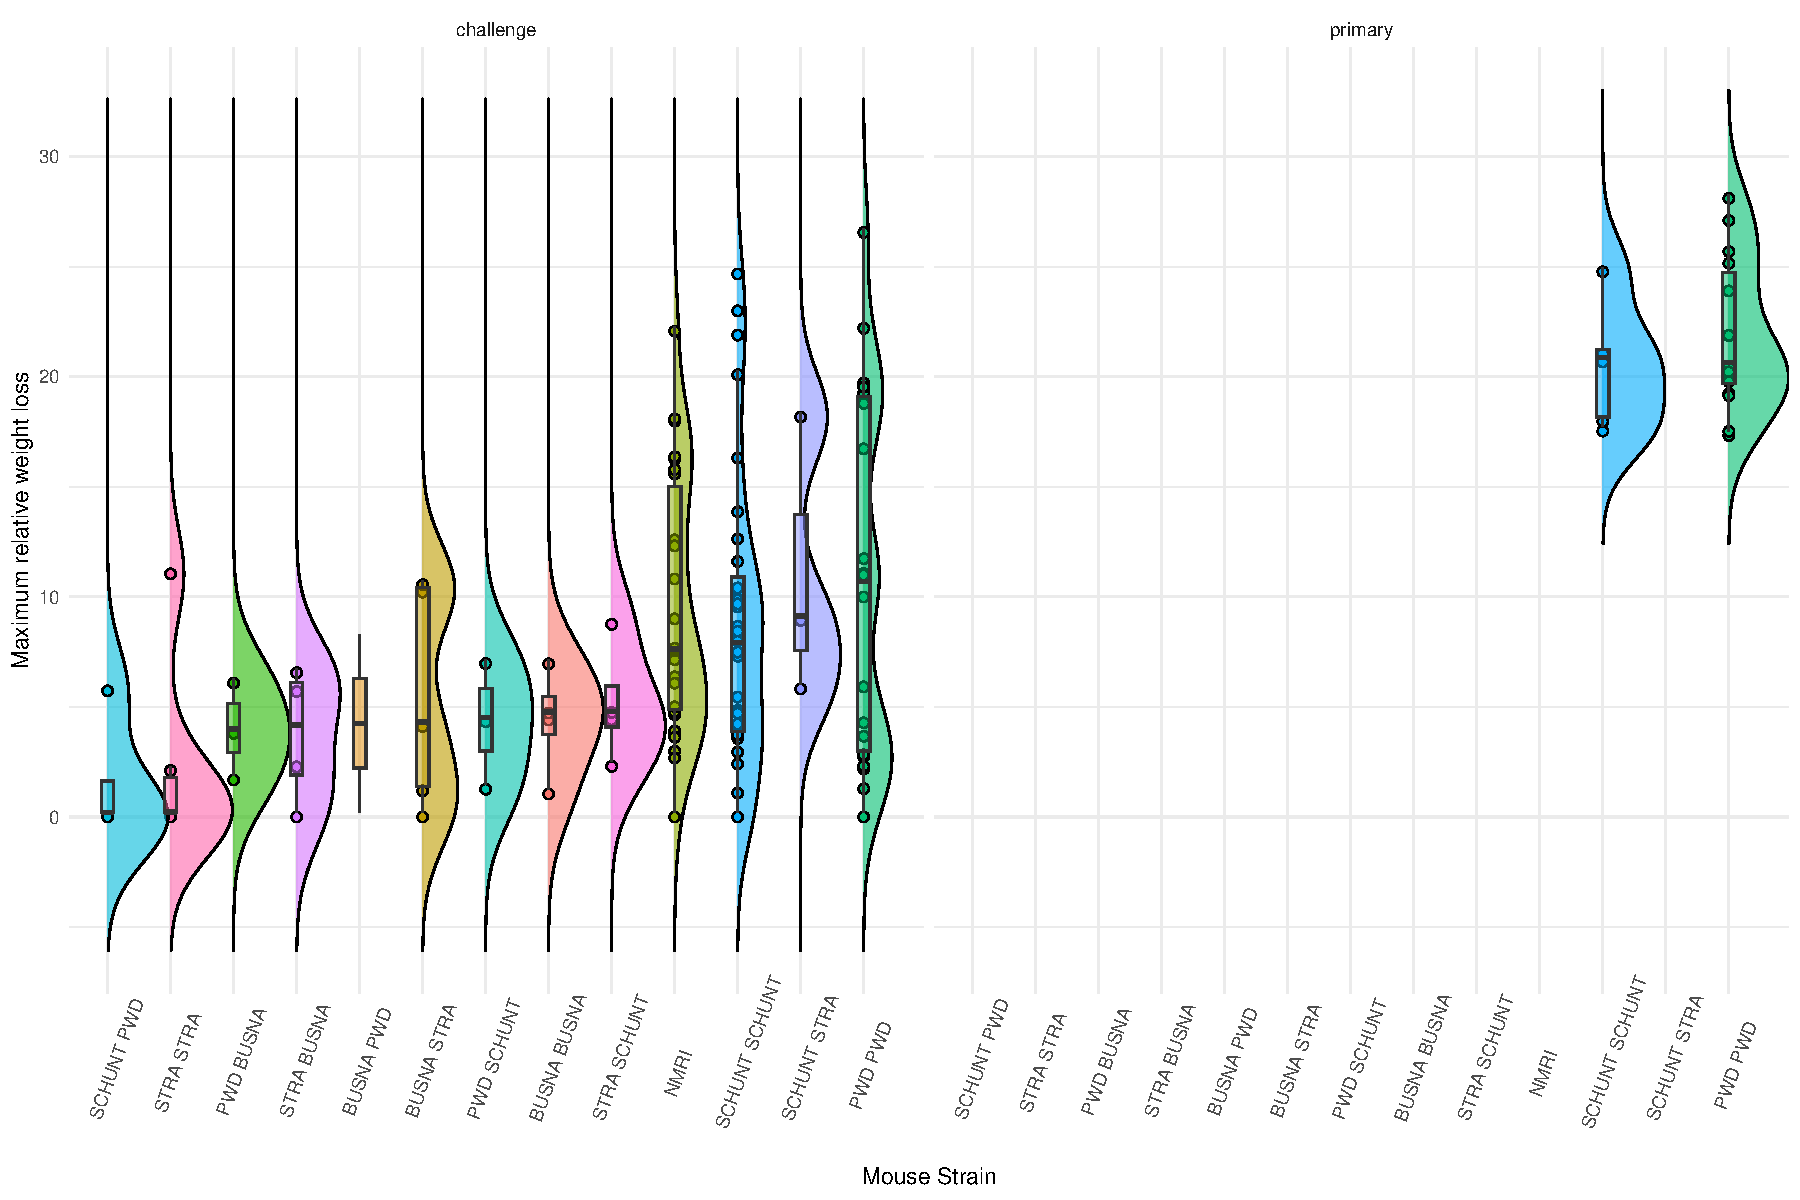
\includegraphics{Explorative_Stats_experimental_planning_files/figure-latex/mouse_strain_WL_chal_prim-1.pdf}

\subsection{Preliminary data analysis immune data from laboratory
infection
experiments}\label{preliminary-data-analysis-immune-data-from-laboratory-infection-experiments}

\subsubsection{For how many mice do we have immune
data?}\label{for-how-many-mice-do-we-have-immune-data}

\begin{Shaded}
\begin{Highlighting}[]
\FunctionTok{length}\NormalTok{(lab}\SpecialCharTok{$}\NormalTok{Mouse\_ID)}
\end{Highlighting}
\end{Shaded}

\begin{verbatim}
## [1] 136
\end{verbatim}

\subsubsection{How many mice in primary and how many in challenge
infections?}\label{how-many-mice-in-primary-and-how-many-in-challenge-infections}

\begin{Shaded}
\begin{Highlighting}[]
\NormalTok{lab }\SpecialCharTok{\%\textgreater{}\%}
    \FunctionTok{group\_by}\NormalTok{(infection) }\SpecialCharTok{\%\textgreater{}\%}
    \FunctionTok{summarize}\NormalTok{(}\FunctionTok{n}\NormalTok{())}
\end{Highlighting}
\end{Shaded}

\begin{verbatim}
## # A tibble: 2 x 2
##   infection `n()`
##   <chr>     <int>
## 1 challenge   116
## 2 primary      20
\end{verbatim}

\subsubsection{How many mice are there in each infection
group?}\label{how-many-mice-are-there-in-each-infection-group}

\begin{Shaded}
\begin{Highlighting}[]
\NormalTok{lab }\SpecialCharTok{\%\textgreater{}\%}
    \FunctionTok{group\_by}\NormalTok{(infection, current\_infection) }\SpecialCharTok{\%\textgreater{}\%}
    \FunctionTok{summarize}\NormalTok{(}\FunctionTok{n}\NormalTok{())}
\end{Highlighting}
\end{Shaded}

\begin{verbatim}
## # A tibble: 6 x 3
## # Groups:   infection [2]
##   infection current_infection `n()`
##   <chr>     <chr>             <int>
## 1 challenge E. falciformis       31
## 2 challenge E. ferrisi           39
## 3 challenge uninfected           46
## 4 primary   E. falciformis       14
## 5 primary   E. ferrisi            5
## 6 primary   uninfected            1
\end{verbatim}

\subsubsection{For how many mice do we have FACS
data?}\label{for-how-many-mice-do-we-have-facs-data}

\begin{verbatim}
## [1] 80
\end{verbatim}

\subsubsection{For how many mice do we have immune gene expression
data?}\label{for-how-many-mice-do-we-have-immune-gene-expression-data}

\begin{verbatim}
## [1] 136
\end{verbatim}

\subsubsection{How many mice have immune gene expression AND FACS
data?}\label{how-many-mice-have-immune-gene-expression-and-facs-data}

\begin{Shaded}
\begin{Highlighting}[]
\FunctionTok{length}\NormalTok{(}\FunctionTok{intersect}\NormalTok{(FACS\_M}\SpecialCharTok{$}\NormalTok{Mouse\_ID, GENE\_M}\SpecialCharTok{$}\NormalTok{Mouse\_ID))}
\end{Highlighting}
\end{Shaded}

\begin{verbatim}
## [1] 80
\end{verbatim}

For the complete FACS Data set, immune gene expression is complete too.

\section{Field infections - FACS immune cell
data}\label{field-infections---facs-immune-cell-data}

\subsubsection{Number of mice with FACS
data}\label{number-of-mice-with-facs-data}

\begin{verbatim}
## [1] 94
\end{verbatim}

\subsubsection{Number of mice with gene expression
data}\label{number-of-mice-with-gene-expression-data}

\begin{verbatim}
## [1] 336
\end{verbatim}

\subsubsection{Capture locations of mice with gene expression
data}\label{capture-locations-of-mice-with-gene-expression-data}

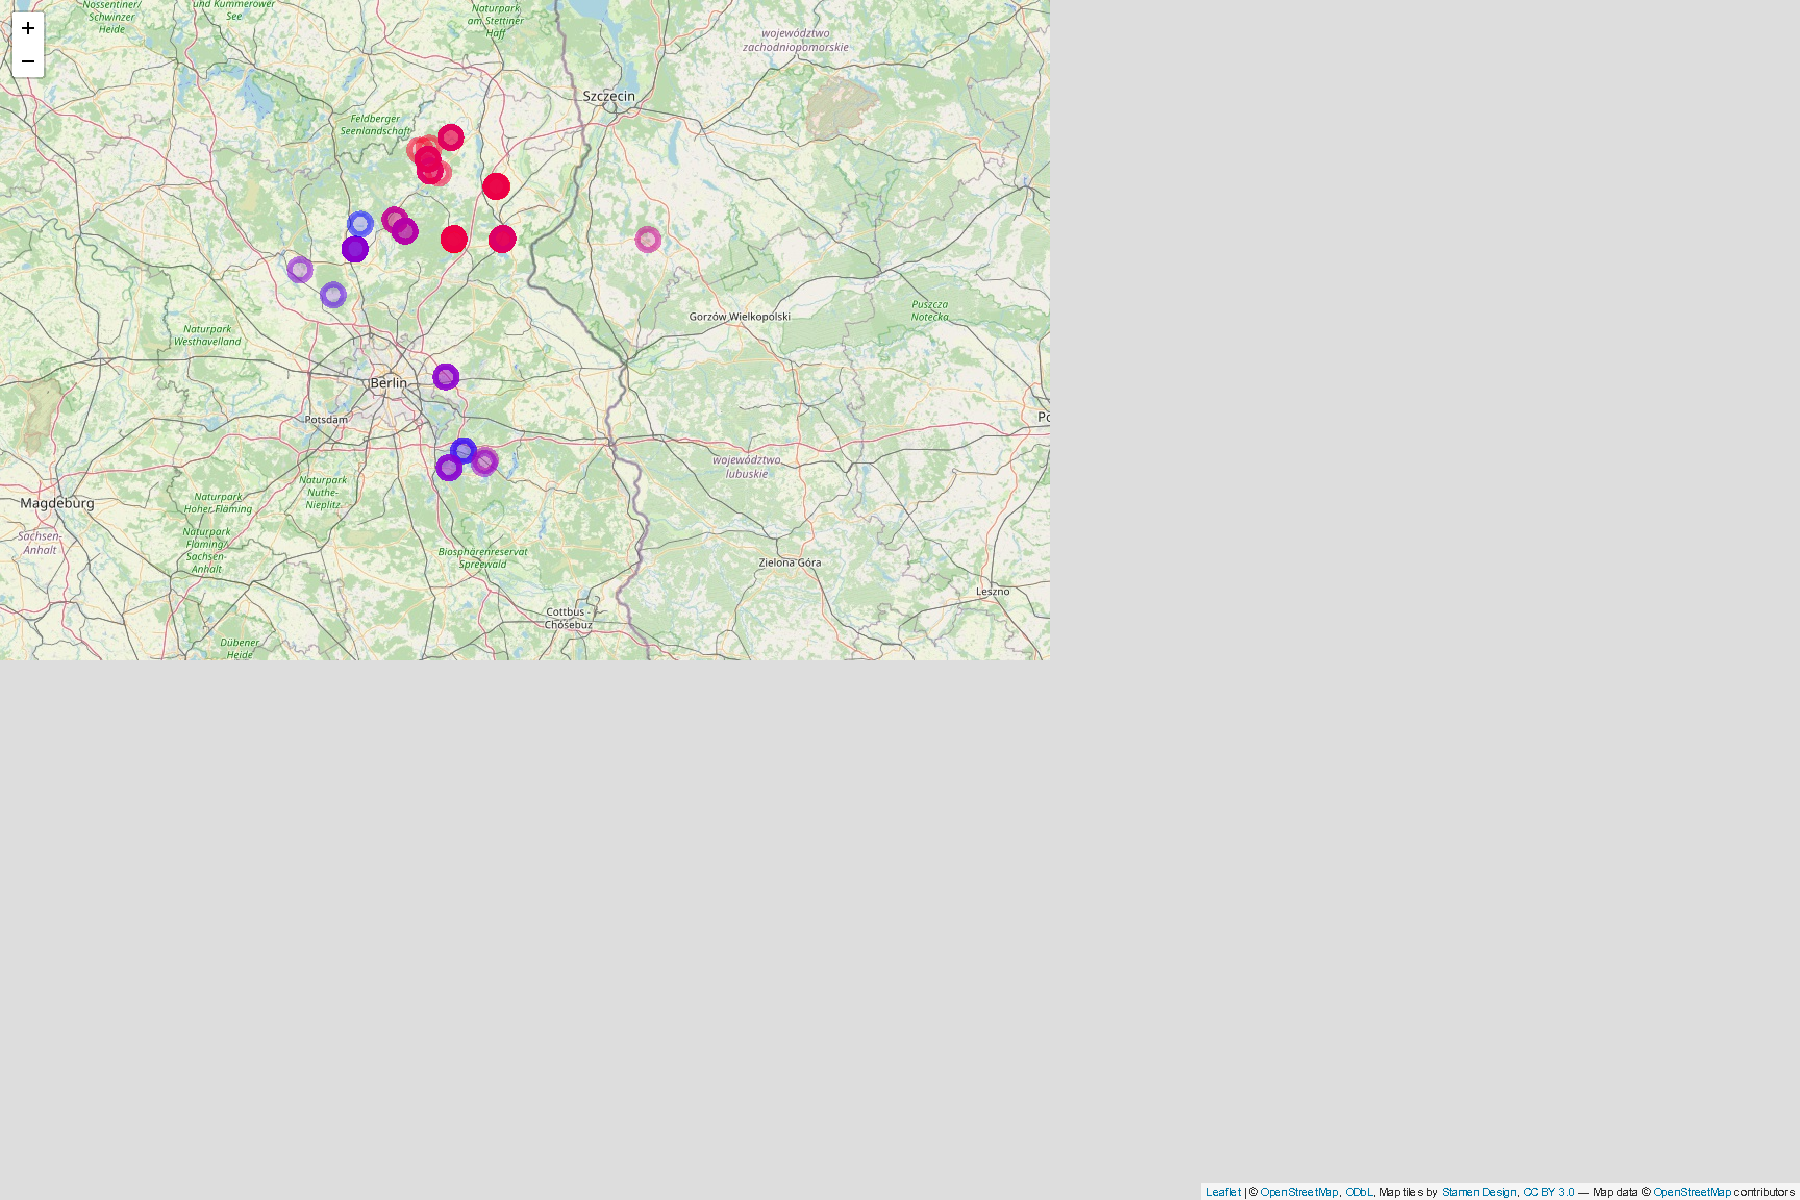
\includegraphics{Explorative_Stats_experimental_planning_files/figure-latex/unnamed-chunk-11-1.pdf}

\subsubsection{Capture locations of mice with immune cell
data}\label{capture-locations-of-mice-with-immune-cell-data}

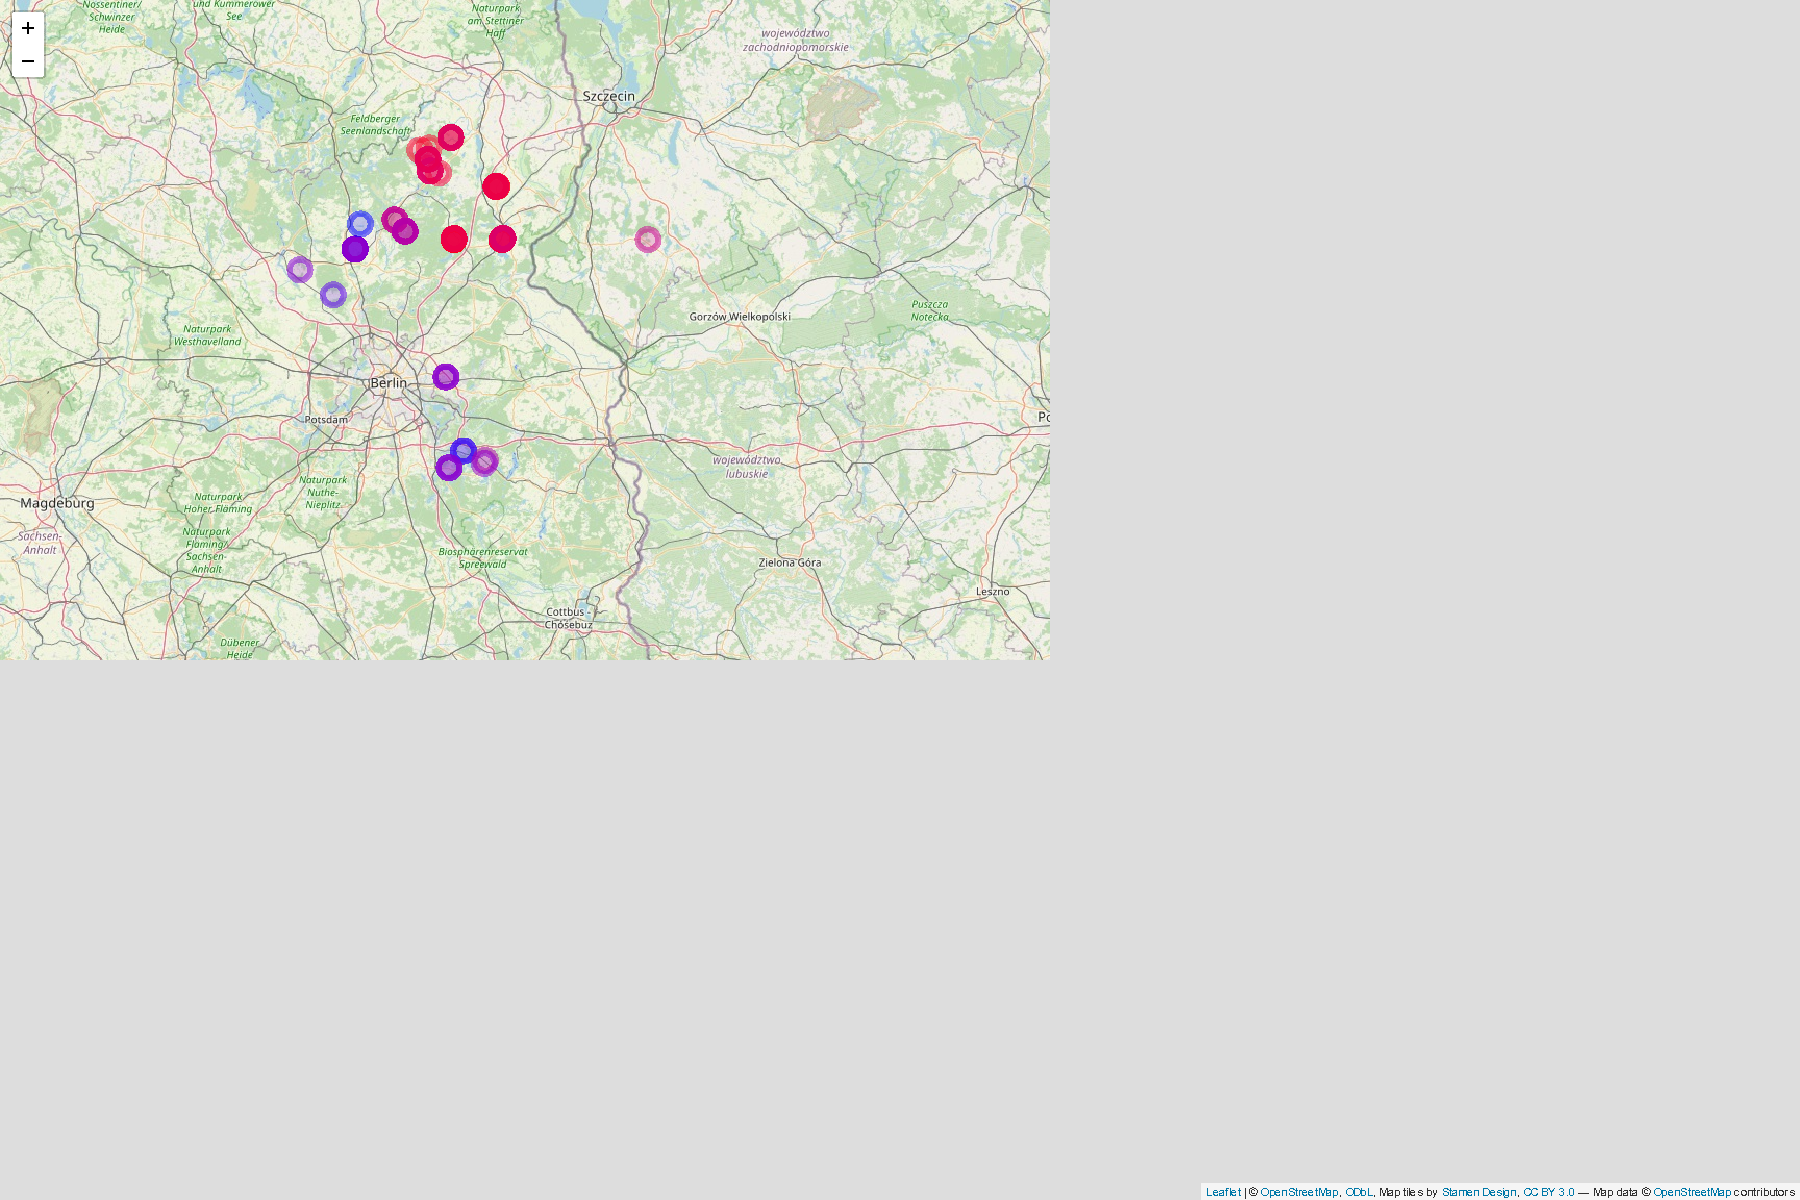
\includegraphics{Explorative_Stats_experimental_planning_files/figure-latex/unnamed-chunk-12-1.pdf}

\subsection{Immune cells}\label{immune-cells}

\subsubsection{Laboratory infections - heatmap of immune
cells}\label{laboratory-infections---heatmap-of-immune-cells}

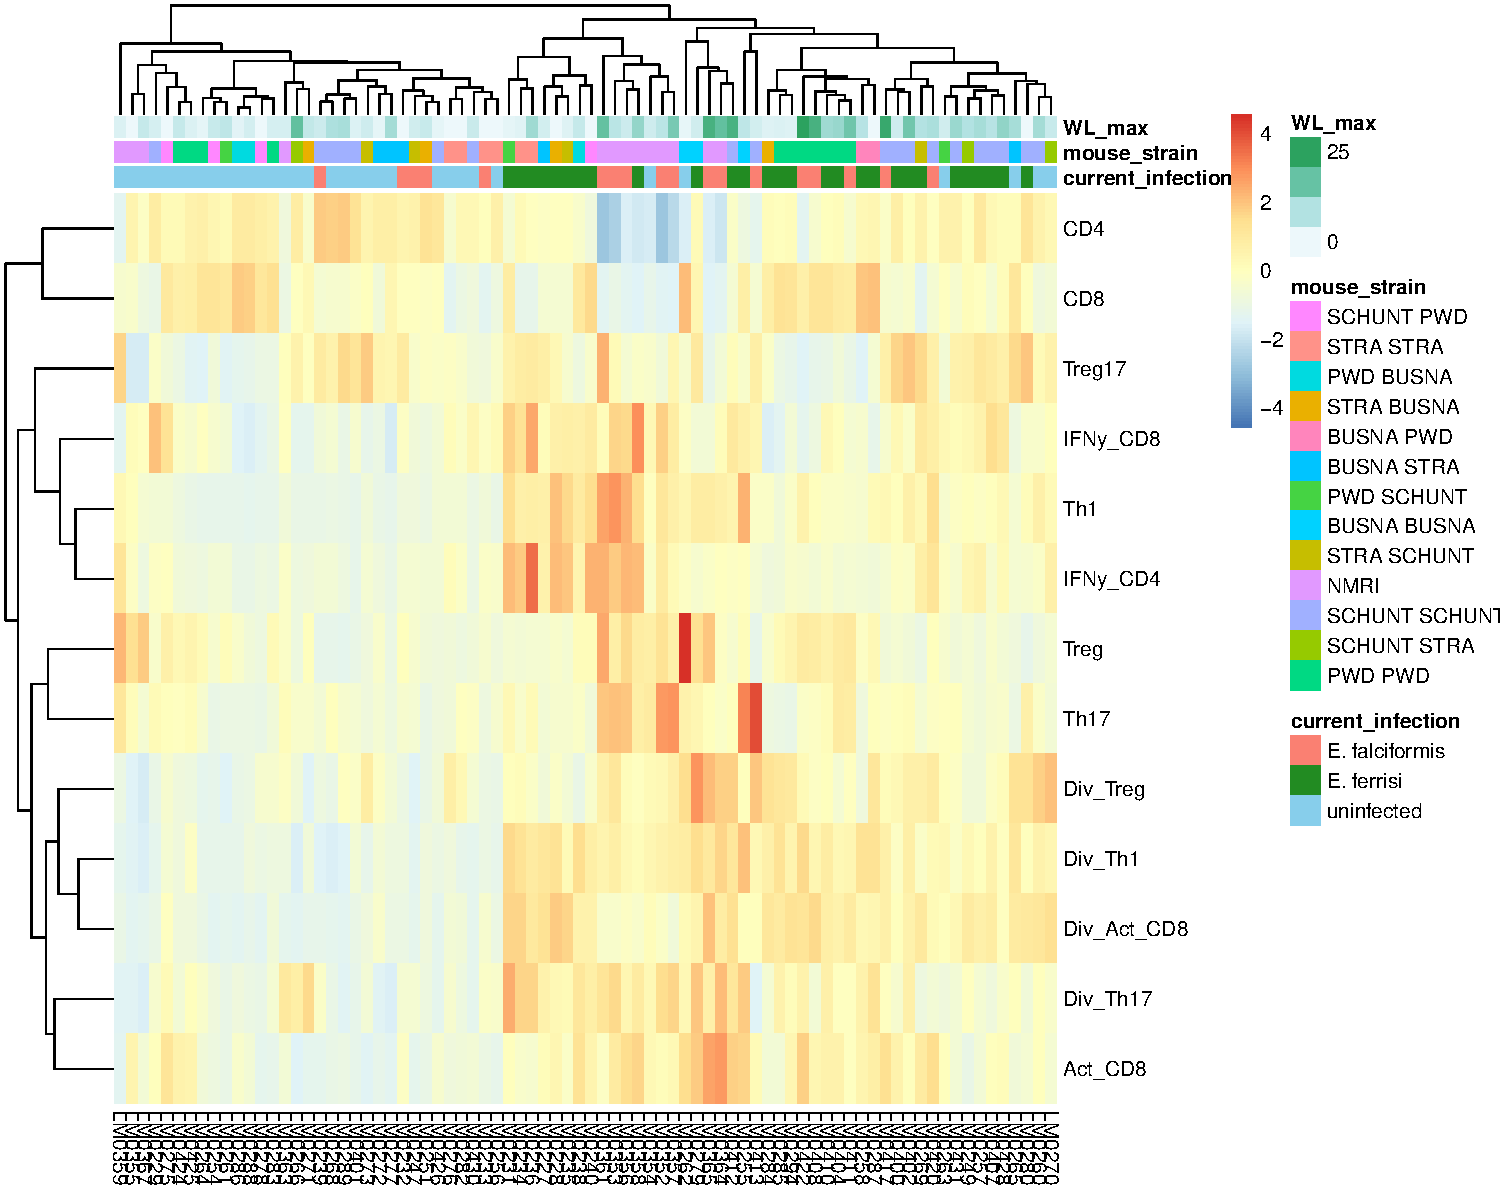
\includegraphics{Explorative_Stats_experimental_planning_files/figure-latex/HEATMAP_lab_facs-1.pdf}

Visual difference between infected and uninfected mice

\subsubsection{Field infections immune cells -
heatmap}\label{field-infections-immune-cells---heatmap}

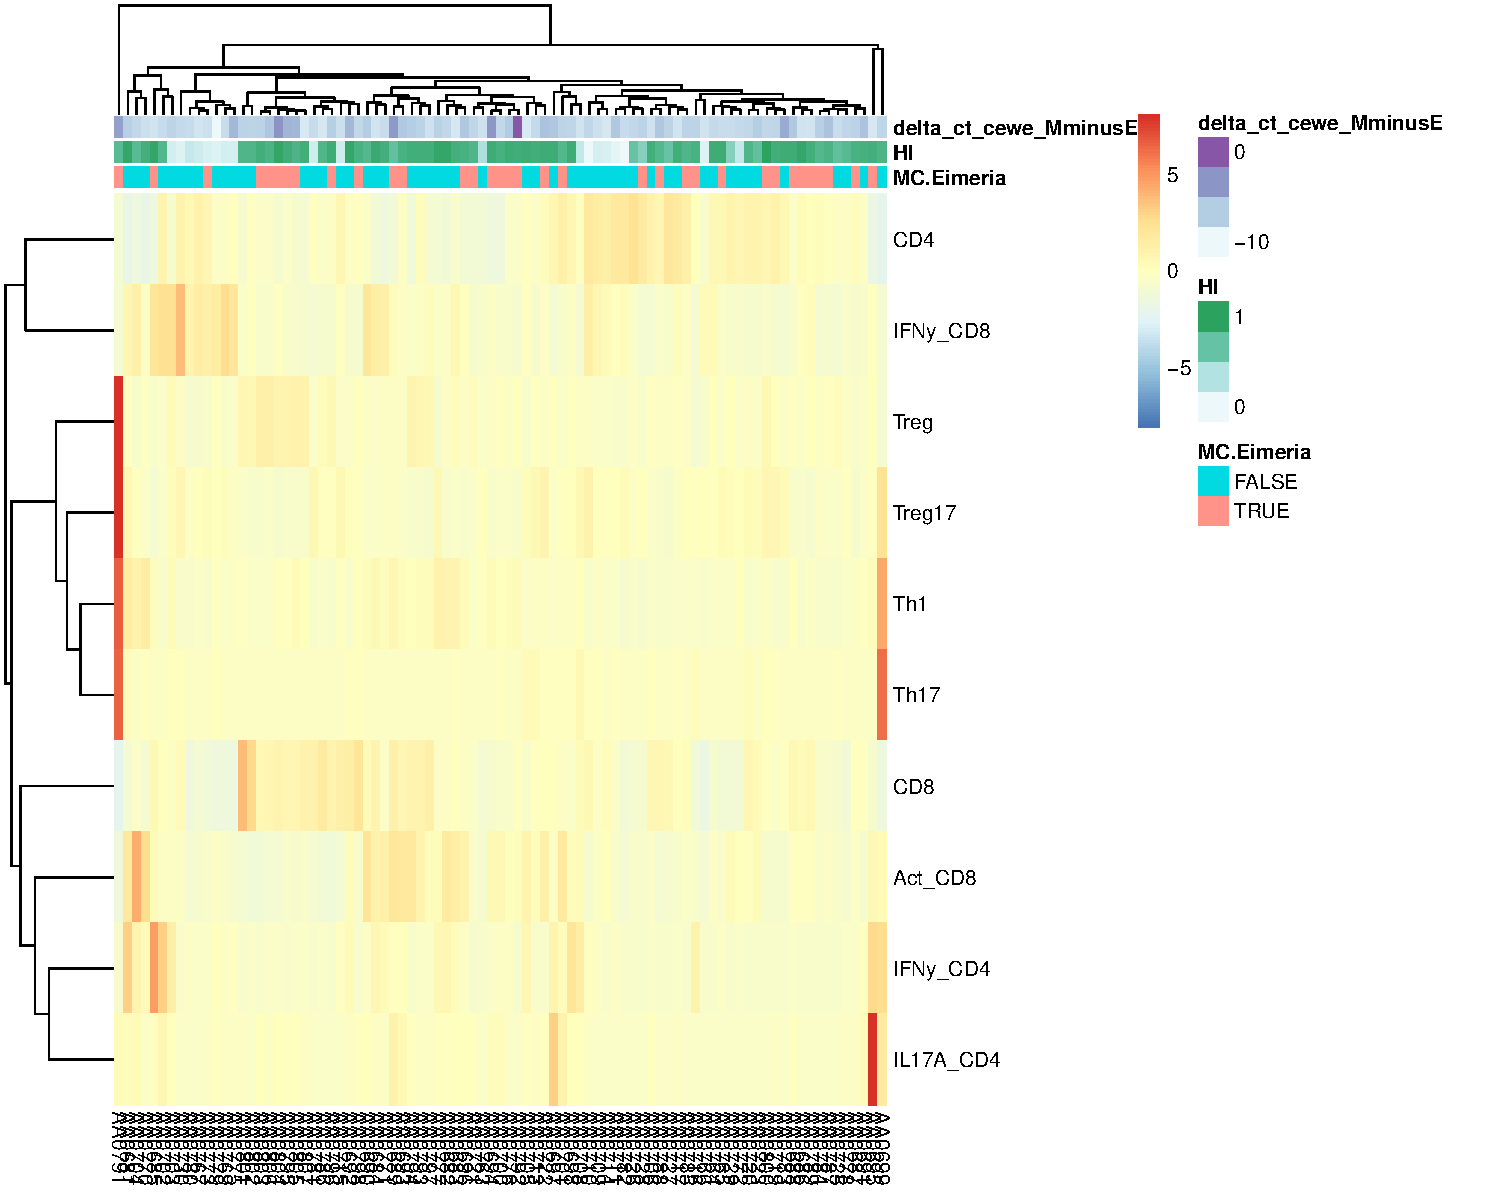
\includegraphics{Explorative_Stats_experimental_planning_files/figure-latex/HEATMAP_field_facs-1.pdf}

Nothing to gain from this

\subsubsection{Correlation between cells in laboratory challenge
infections}\label{correlation-between-cells-in-laboratory-challenge-infections}

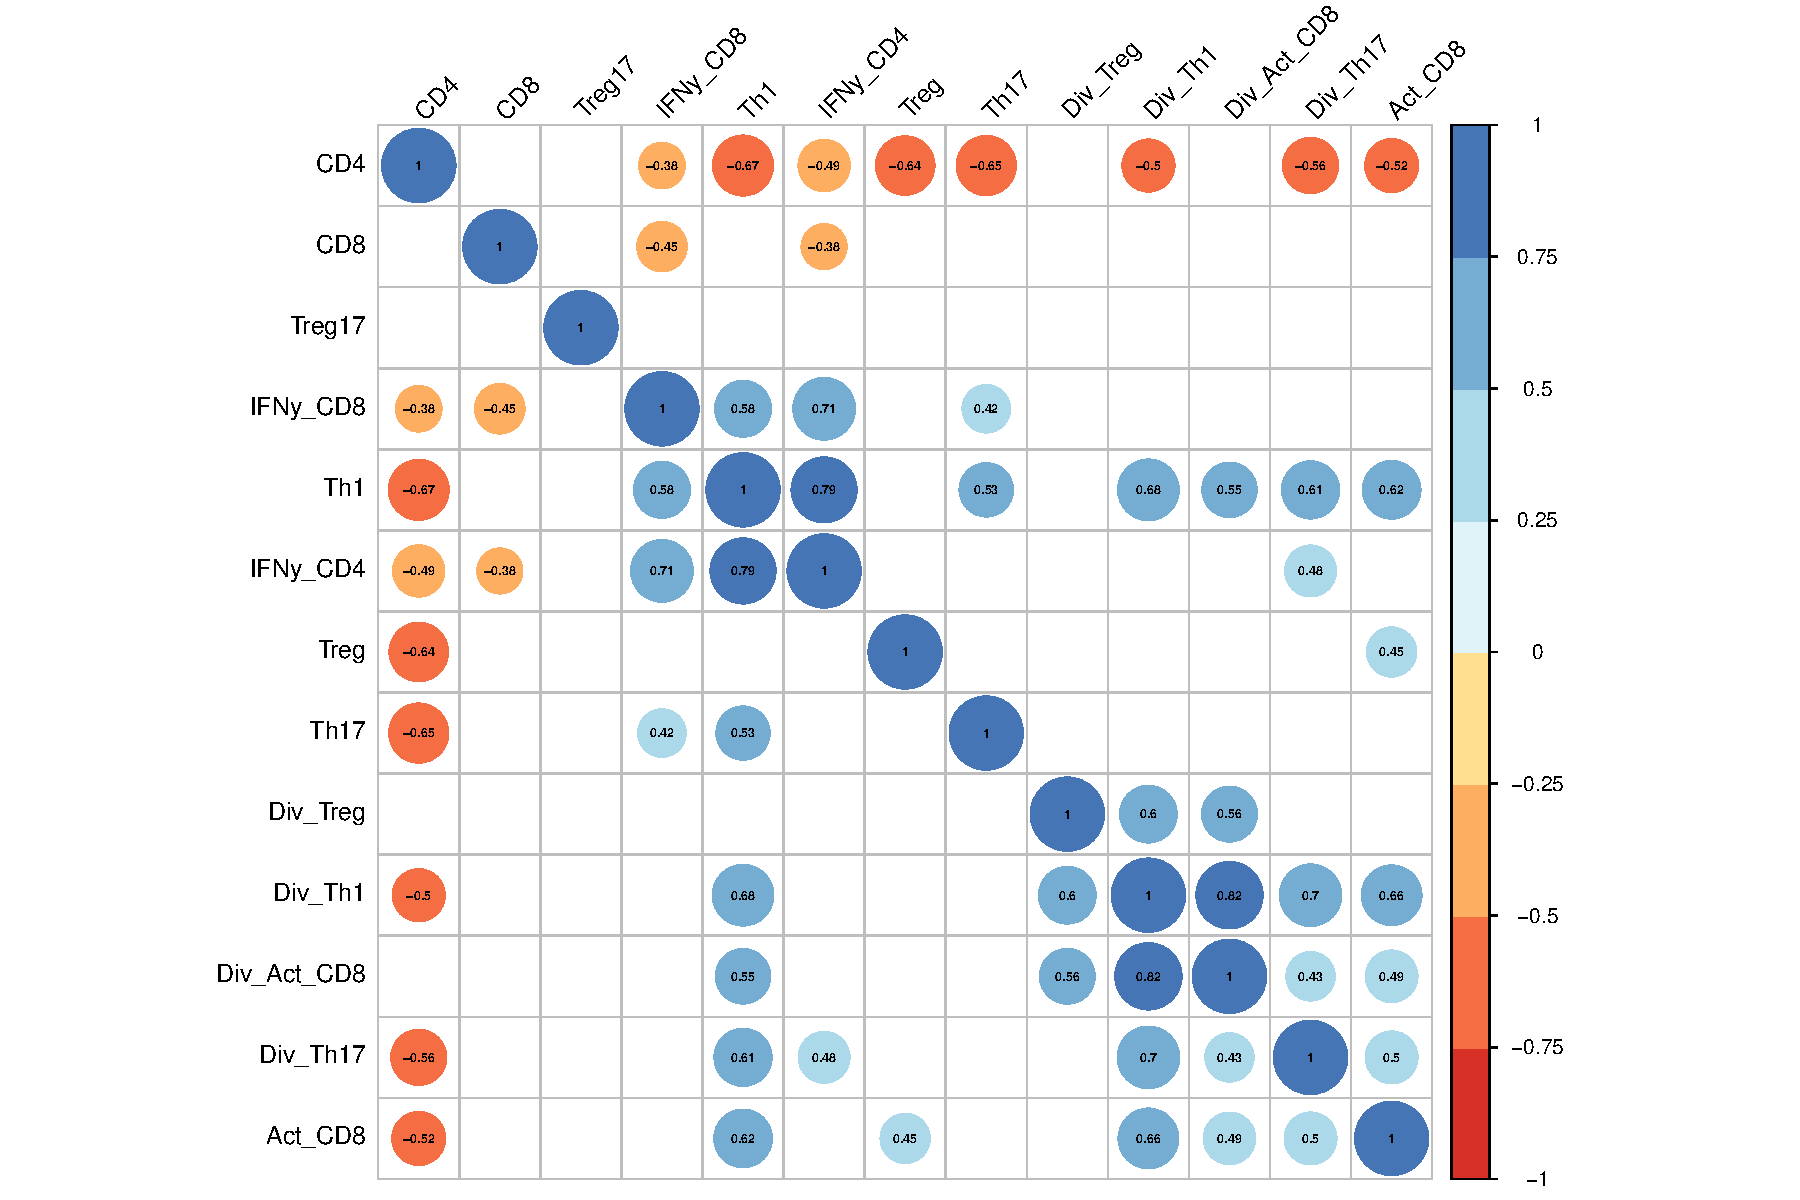
\includegraphics{Explorative_Stats_experimental_planning_files/figure-latex/facs_core-1.pdf}
\#\#\# Correlations between cells in field mice

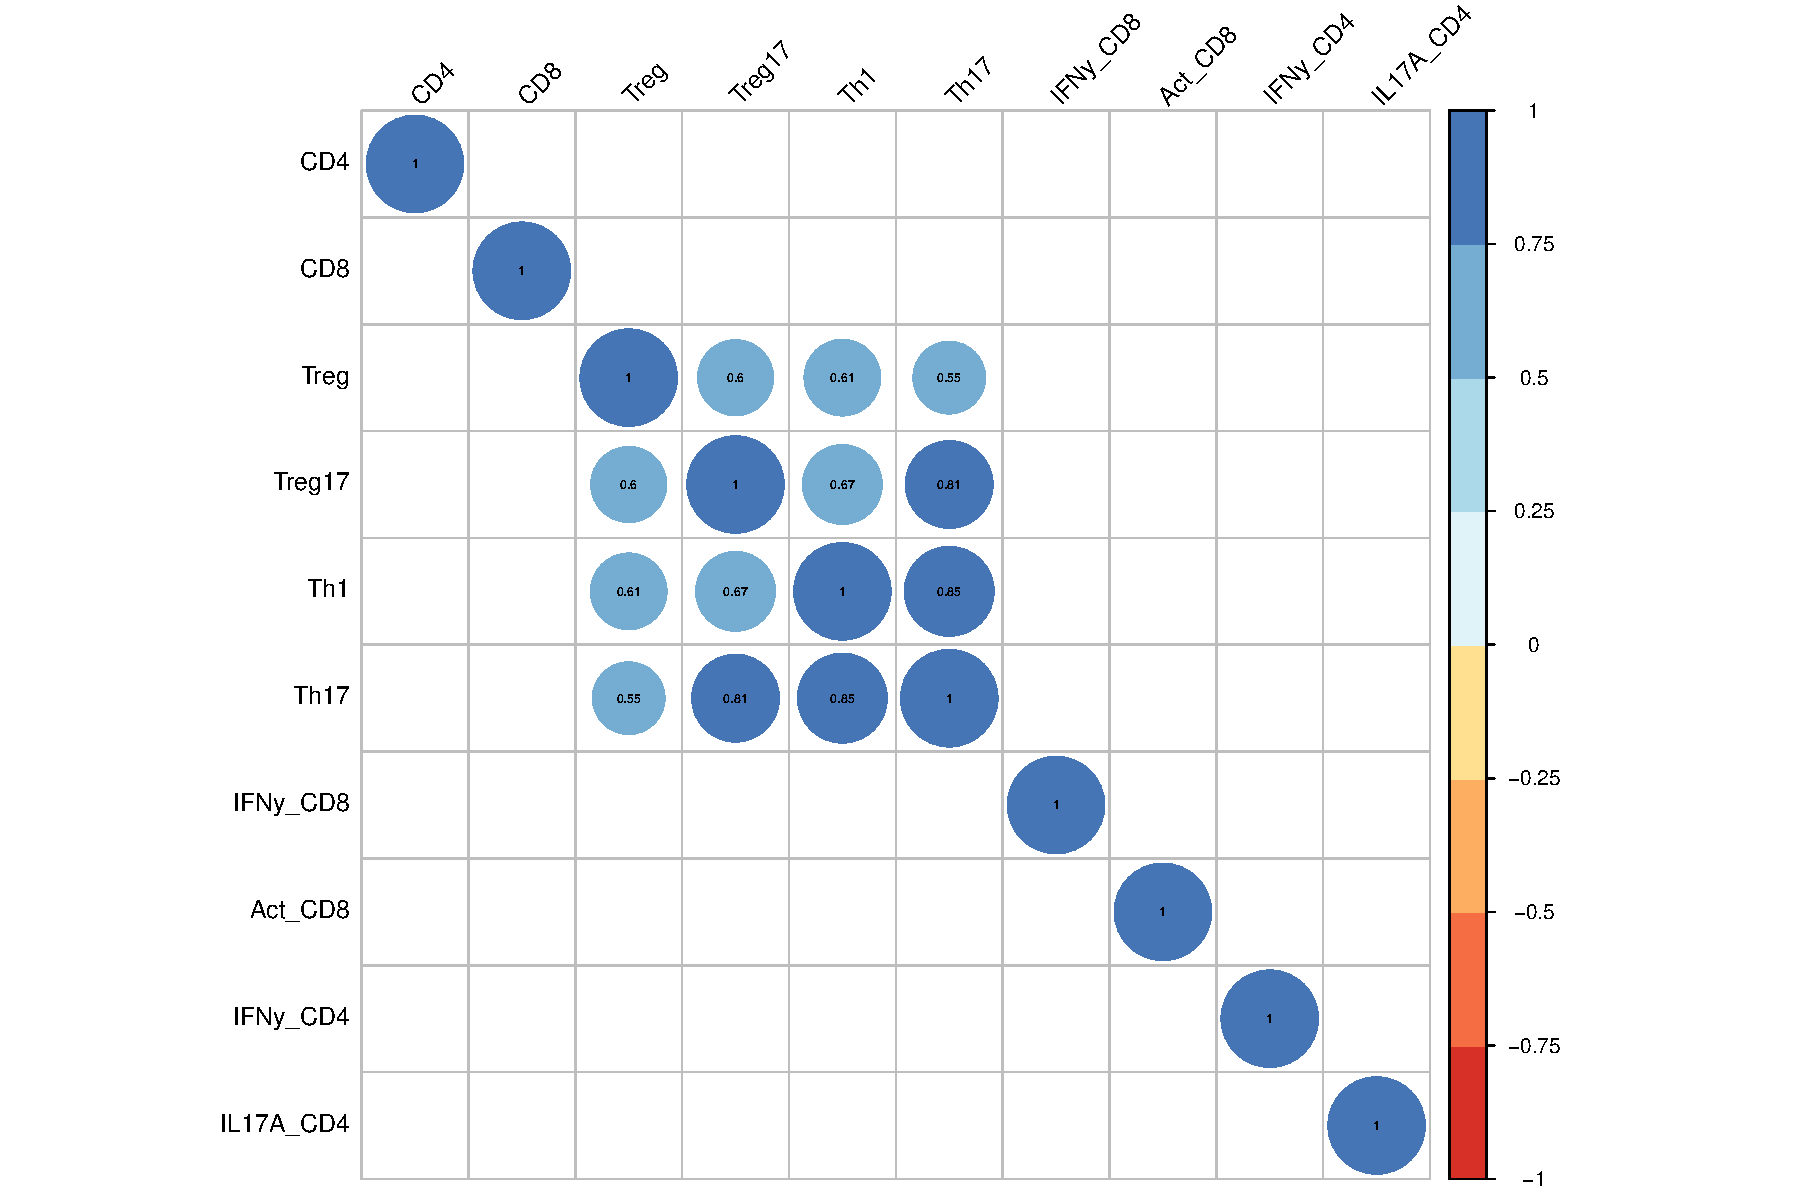
\includegraphics{Explorative_Stats_experimental_planning_files/figure-latex/facs_core_field-1.pdf}

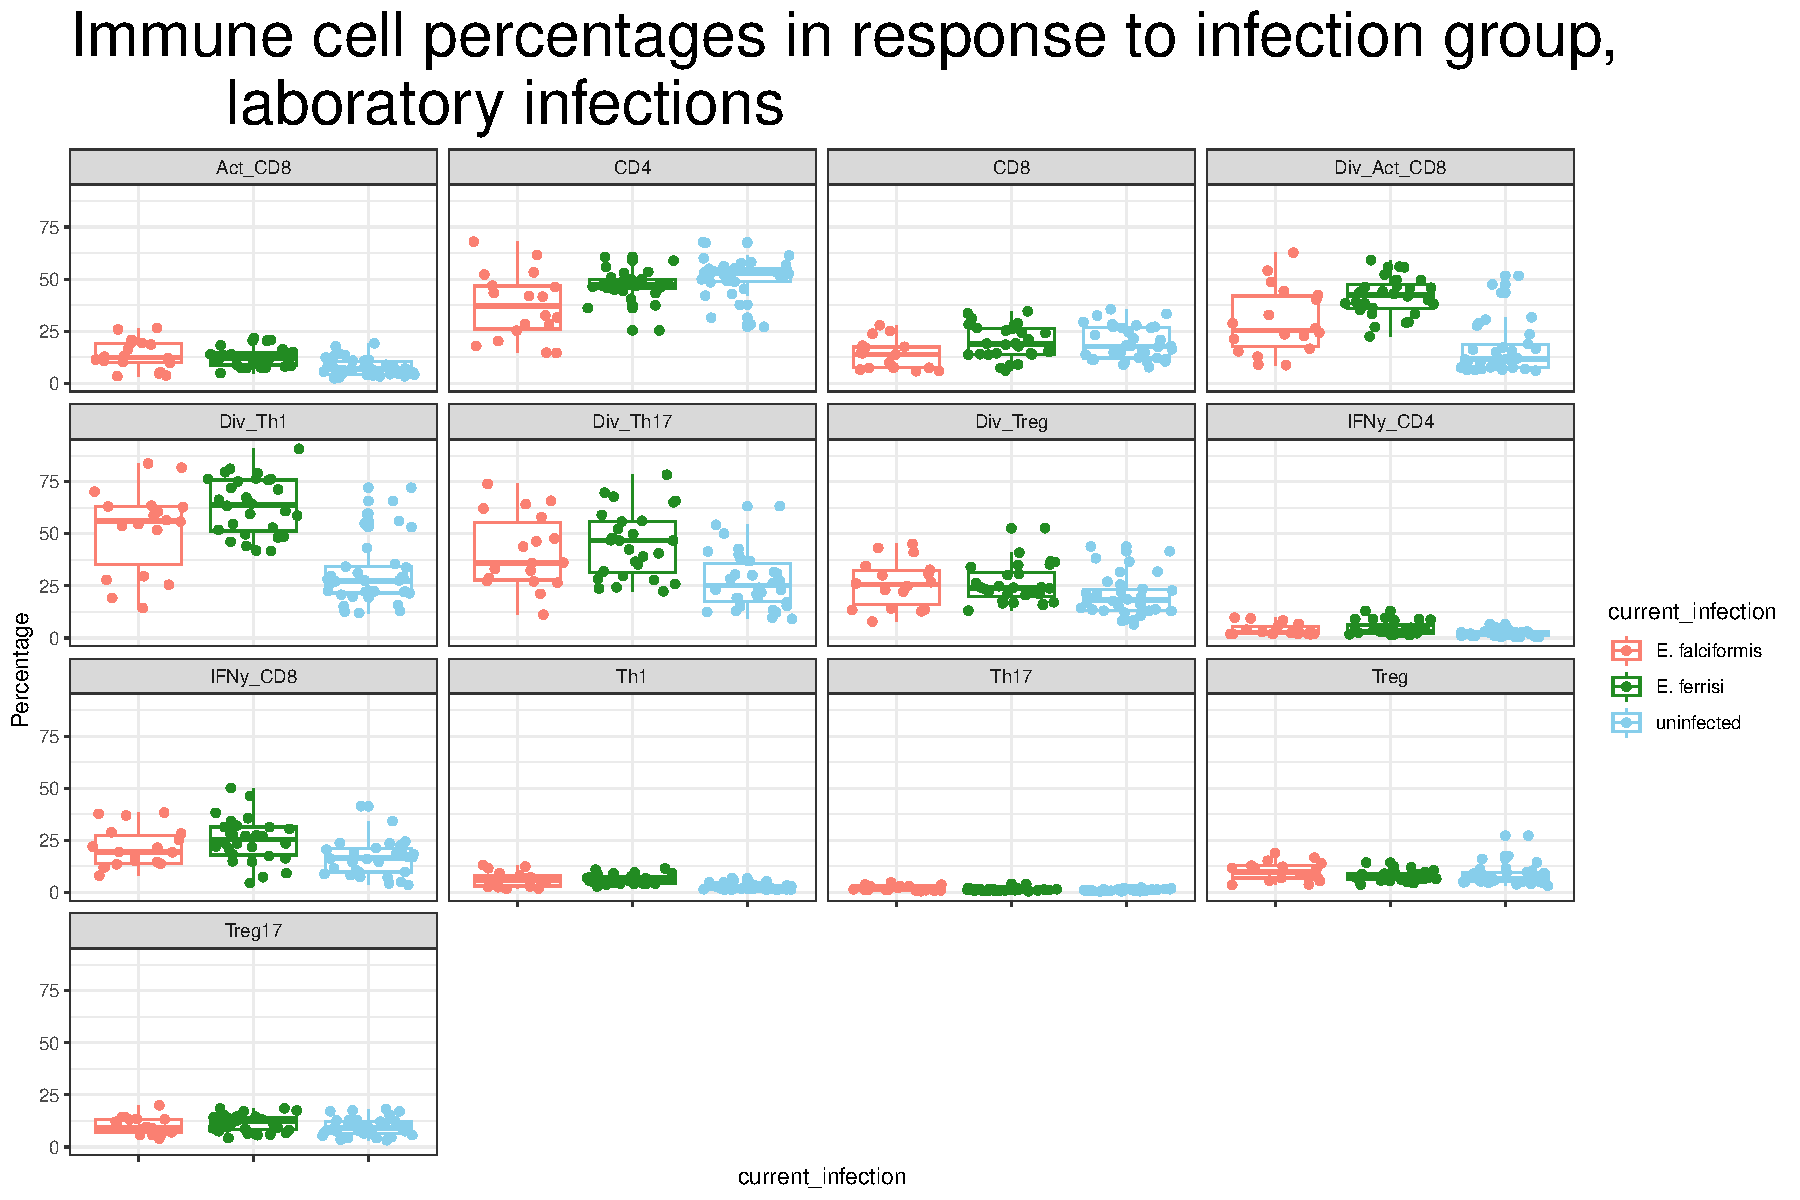
\includegraphics{Explorative_Stats_experimental_planning_files/figure-latex/immune_cells_differences_status-1.pdf}

\begin{itemize}
\tightlist
\item
  Missing: completing the data set of genotyping parasites in field
  samples
\end{itemize}

\end{document}
